\documentclass{article}
\usepackage{tikz}

\begin{document}

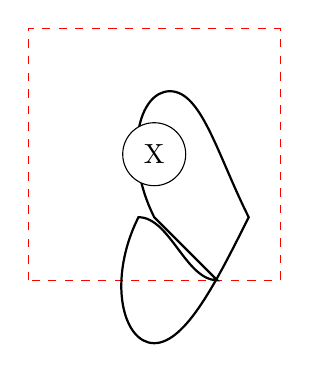
\begin{tikzpicture}[scale=0.8]
    % Draw the bounding box
    \draw[red, dashed] (0,0) rectangle (4,4);
    
    % Draw the shape inside the bounding box
    \draw[thick] (2,1) .. controls (1.5,2) and (1.75,3) .. (2.25,3) .. controls (2.75,3) and (3,2) .. (3.5,1) .. controls (3,0) and (2.5,-1) .. (2,-1) .. controls (1.5,-1) and (1.25,0) .. (1.75,1) .. controls (2.25,1) and (2.5,0) .. (3,0) -- cycle;
    
    % Draw the circle with 'X' in the center
    \draw[fill=white] (2,2) circle (0.5);
    \node at (2,2) {X};
\end{tikzpicture}

\captionof{figure}{Normal bounding box}
\label{fig:normal_bounding_box}

\end{document}